\section{Koord Language and Overview}
\label{sec:semantics}
The interaction model of an agent executing a $\lgname$ program is shown in \reffig{arch}. 
\begin{figure}[!htbp]
\centering
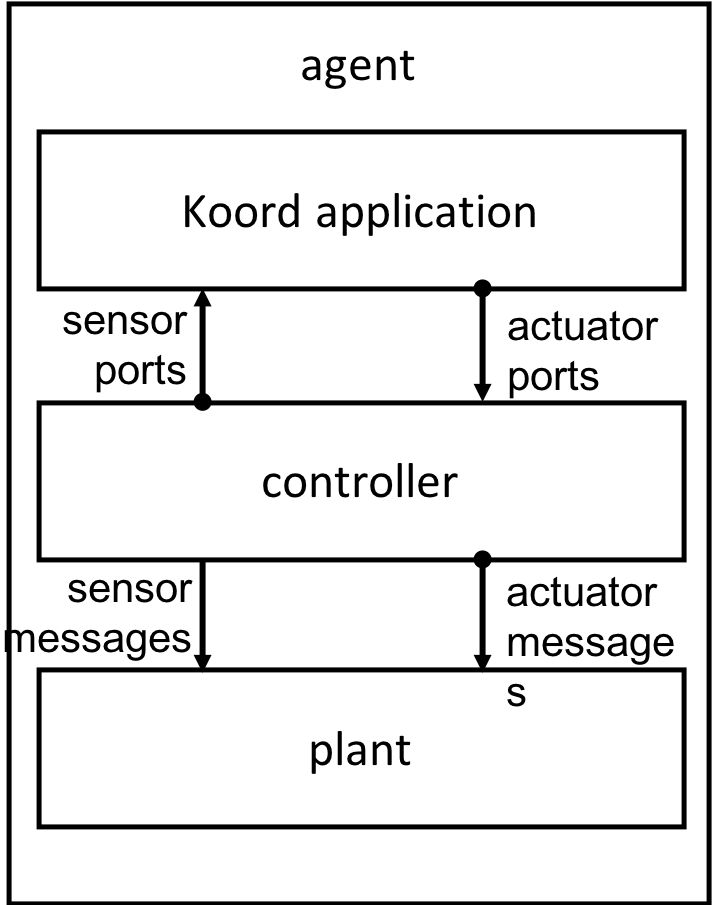
\includegraphics[width=0.23\textwidth]{figs/arch.png}
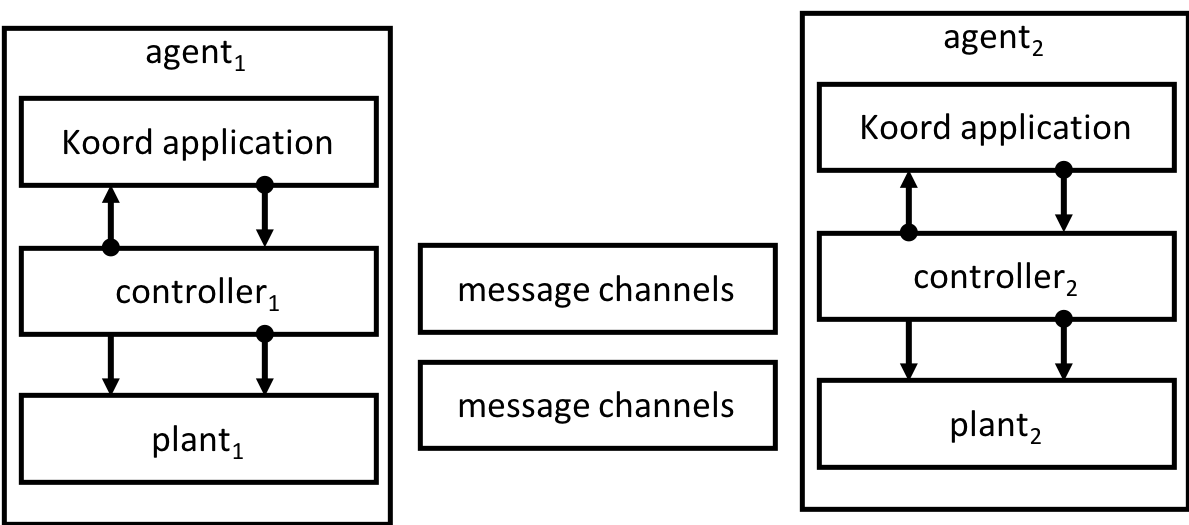
\includegraphics[width=0.24\textwidth]{figs/agents2.png}
\caption{\small An agent executing a $\lgname$ application and interacting with the physical environment through sensor and actuator ports ({\em left}). Interaction across multiple agents happens through shared variables implmented over message passing ({\em right}).}
\label{fig:arch}
\end{figure}
The program and the controller interact with each other through {\em sensor} and {\em actuator} ports.  The program reads the sensor ports, reads and writes to program variables, and writes to actuator ports. The controller drives the underlying physical plant. The \emph{environment} of a  $\lgname$ program is the combination of the controller and the plant. The set of agents in the system may interact with each other using {\em shared variables\/}. Each agent in the system runs an instance of the \emph{same} $\lgname$ program. 
% exmaple code snippet
\begin{figure}[!htbp]
    \noindent
    \begin{mdframed}

    \begin{center}
        \scriptsize
        \two{0.4}{0.6}
        {\lstinputlisting[language=xyzNums,firstline=1,lastline=23,frame=none]{code/mapapp.tex}}
        {\lstinputlisting[language=xyzNums,firstline=24,frame=none,firstnumber=24]{code/mapapp.tex}}
    \end{center}
    \end{mdframed}

    \caption{$\lgname$ program for robot $i$ to perform distributed mapping}
    \label{fig:mapapp}
\end{figure}
    
\paragraph* {A distributed $\mathit{Mapping}$  application} \reffig{mapapp} shows a distributed mapping allocation application written in $\lgname$. This app involves :
\begin{itemize}
    \item Multiple sensors
    \item Sampled sensing : sensed over time. 
    \item Coordination using shared variables. 
    \item Mutual exclusion. 
\end{itemize}
% language features - what main "issue" each feature addresses . 

\subsection{Koord model for distributed CPS}


$\lgname$ design comprises of a \emph{turn}-based alternating semantics of discrete and dynamic behavior of each agent in the distributed system. The agents can be viewed as performing \emph{rounds} of execution, where each round consists of a \begin{inparaenum} 
\item \emph{a program transition} which is a discrete computational step, and 
\item \item \emph{an environment transition} which is the dynamic behavior of the controller, environment, and their effect on the sensors and actuators
\end{inparaenum}. 

In a program transition in a round, each agent first  chooses an \emph{enabled} event, or an event whose precondition evaluates to \verb|True|. It then executes the statements in the effect of that event. %This may involve reading sensor ports, performing computations using local and shared variables, and writing to actuator ports. 
Then, the agent performs the environment transition in the round, during which it interacts with the physical environment and behaves as dictated by the actuator ports on the controller for $\delta$ amount of time.  \footnote{ $\delta>0$ is a constant \emph{sampling period} parameter. The sampling parameter can be provided by the user, and each controller that $\lgname$ supports has a default sampling parameter which has been set based on the experiments using the controller. See \refsect{experims} for more details.}  %During this time, the program variables and the actuator port values remain constant, the state of the environment (controller and plant) and the values of the sensor ports change according to the dynamics of the environment.

The controller which determines the dynamic behavior of each agent and its interaction with the environment. The agent program can read from the sensor ports read and write to the actuator ports during the program transition. The sensor ports are updated during the environment transition according to the controller dynamics. 


As our design choices impose this synchronicity on all agent executions, the system can also be seen to be executing program and environment transitions by \emph{turns}, where all the agents execute the environment transitions in a round only after all of them have finished executing the program transitions in that round (in some order). 

 
\subsection{Program (cyber) variables and physical variables}
\label{sec:variables}
We first introduce the types of variables used by the $\lgname$ programs. 

\paragraph{Program variables}
%$\lgname$ provides several types of access for program variables. 
An agent's $\lgname$ program can access three types of variables. 
%
\begin{itemize}
	\item {\em Local program variables\/} record the state of the program. 
\item {\em Distributed shared variables\/} are used for communication across agents.  For example, {\bf allwrite} $\mathit{taskList}$ (Line~\ref{awvar}) is a multi-writer list of tasks which can be written-to and read-from by all participating agents. Shared variables can also be single-writer multi-reader ({\bf allread}). For each shared variable, an agent maintains a {\em local copy\/}  of the variable. 

\item {\em Port variables\/} are used to read from and write to sensor and actuator ports of the agent. For example, the $\mathit{Motion}$ controller for the $\mathit{Mapping}$ app  drives the agent  to a point, as directed by value set at the actuator port $\mathit{Motion.target}$. The sensor port $\mathit{Motion.psn}$ gives the position of the agent (in a fixed coordinate system) and $\mathit{Motion.reached}$ indicates  whether the $\mathit{Motion}$ controller is active or inactive.
\end{itemize}

%Also, should 
The agent program also has access to two system-level constant parameters (a) a unique integer identifier $\myuin$ for itself and (b) a list $\UINS$ of identifiers of all participating agents\footnote{Our current system implementation assumes that the set of possible participating agents is known. This assumption will be relaxed in the future.}. 


